\section{Dataset Analysis} \label{sec:analysis}

In this section, we analyze the types of questions, types of answers, and types of multi-hop reasoning covered in the dataset.

\begin{figure}[!t]
    \centering
    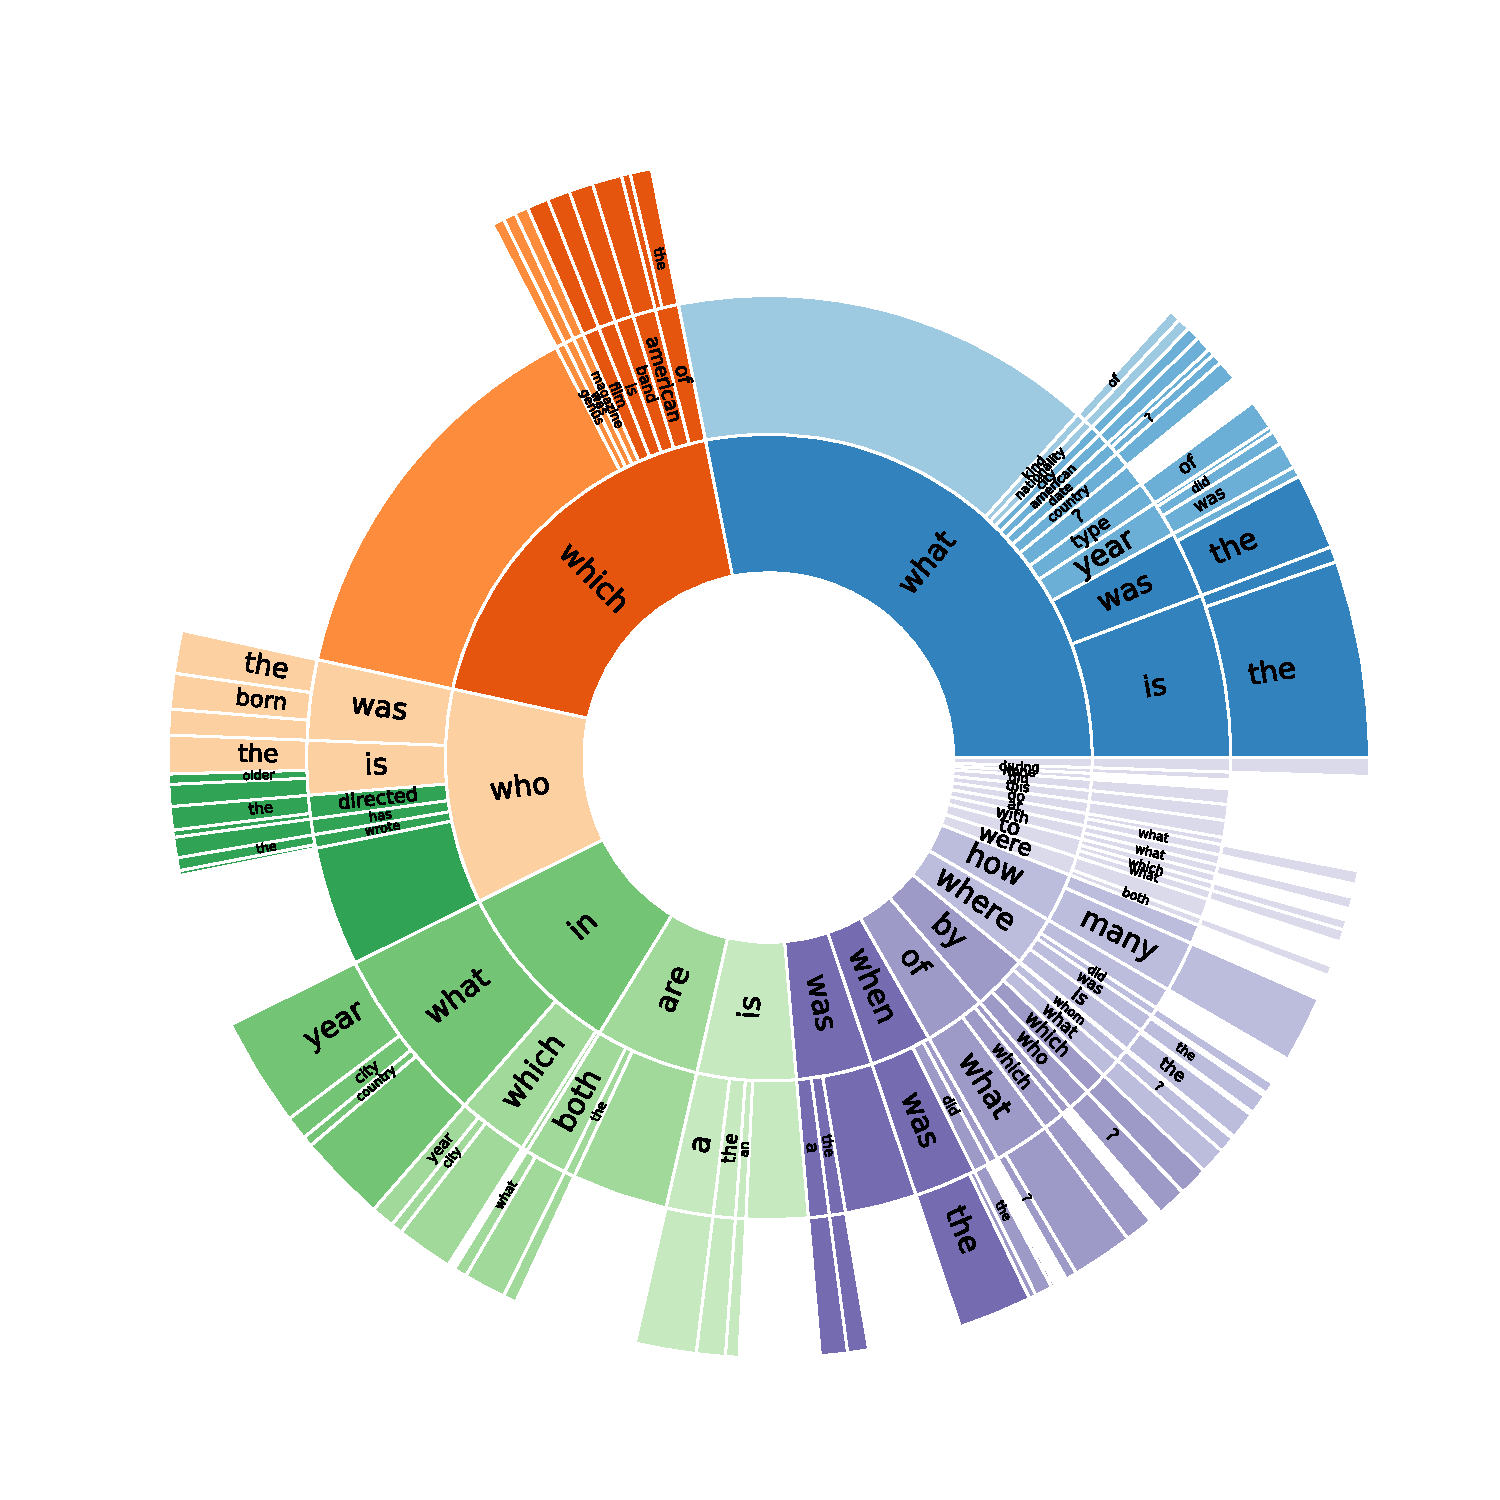
\includegraphics[width=.48\textwidth]{images/question_types}
    \vskip -0.7em
    \caption{Types of questions covered in \datasetname{}. Question types are extracted heuristically, starting at question words or prepositions  preceding them. Empty colored blocks indicate suffixes that are too rare to show individually. See main text for more details.} \label{fig:question_types}
    % \vskip -1em
\end{figure}

\paragraph{Question Types.}
We heuristically identified question types for each collected question.
% , and present the aggregated statistics in Figure \ref{fig:question_types}.
To identify the question type, we first locate the \emph{central question word} (CQW) in the question.
Since \datasetname{} contains comparison questions and yes/no questions, we consider as \emph{question words} WH-words, copulas (``is'', ``are''), and auxiliary verbs (``does'', ``did'').
Because questions often involve relative clauses beginning with WH-words, we define the CQW as the first question word in the question if it can be found in the first three tokens, or the last question word otherwise.
Then, we determine question type by extracting words up to 2 tokens away to the right of the CQW, along with the token to the left if it is one of a few common prepositions (e.g., in the cases of  ``in which'' and ``by whom'').

We visualize the distribution of question types in Figure \ref{fig:question_types}, and label the ones shared among more than 250 questions.
As is shown, our dataset covers a diverse variety of questions centered around entities, locations, events, dates, and numbers, as well as yes/no questions directed at comparing two entities (``Are both A and B ...?''), to name a few.



\paragraph{Answer Types.}
We further sample 100 examples from the dataset, and present the types of answers in Table \ref{tab:answer_types}.
As can be seen, \datasetname{} covers a broad range of answer types, which matches our initial analysis of question types.
We find that a majority of the questions are about entities in the articles (68\%), and a non-negligible amount of questions also ask about various properties like date (9\%) and other descriptive properties such as numbers (8\%) and adjectives (4\%).

\begin{table}[!t]
    \centering
    \small
    \begin{tabular}{p{2cm}rp{4.2cm}}
        \toprule
        Answer Type & \% & Example(s) \\
        \midrule
        Person & 30 & King Edward II, Rihanna \\
        Group / Org & 13 & Cartoonito, Apalachee \\
        Location & 10 & Fort Richardson, California \\
        Date & 9 & 10th or even 13th century\\
        Number & 8 & 79.92 million, 17 \\
        Artwork & 8 & Die schweigsame Frau \\
        Yes/No & 6 & - \\
        Adjective & 4 & conservative \\
        Event & 1 & Prix Benois de la Danse \\
        Other proper noun & 6 & Cold War, Laban Movement Analysis \\
        Common noun & 5 & comedy, both men and women\\
        % Person & 29 & King Edward II, Rihanna \\
        % Group / Organization & 13 & British Army, Apalachee \\
        % Location & 12 & Fort Richardson \\
        % Date & 6 & 10th or even 13th century, 1994\\
        % Event & 2 & SXSW, Burning Man \\
        % Number & 2 & 79.92 million \\
        % Adjective & 2 & conservative \\
        % Yes-no & 2 &\\
        % Other proper noun & 18 & Cold War, The Frog Princess \\
        % Common noun & 12 & comedy, both men and women\\
        \bottomrule
    \end{tabular}
    \vskip -0.7em
    \caption{Types of answers in \datasetname{}.} \label{tab:answer_types}
    % \vskip -1em
\end{table}

\begin{table*}[!t]
    \centering
    \small
    \begin{tabular}{p{2.9cm}rp{11.7cm}}
        \toprule
        Reasoning Type & \% & Example(s) \\
        \midrule
        % type 2
        Inferring the \bridge{bridge entity} to complete the 2nd-hop question (Type I) & 42 &
        \textbf{Paragraph A:} The 2015 Diamond Head Classic was a college basketball tournament ...  \bridge{Buddy Hield} \support{was named the tournament's MVP}.\newline
        \textbf{Paragraph B:} \bridge{Chavano Rainier "Buddy" Hield} is a Bahamian professional basketball player for the \answer{Sacramento Kings} of the NBA... \newline
        \textbf{Q:}  Which team does the player named 2015 Diamond Head Classic's MVP play for?
        \\
        \midrule
        % type 4
        Comparing two entities (Comparison) & 27 &
        \textbf{Paragraph A:} LostAlone were a British rock band ... consisted of \support{Steven Battelle, Alan Williamson, and Mark Gibson}... \newline
        \textbf{Paragraph B:} Guster is an American alternative rock band ... Founding members \support{Adam Gardner, Ryan Miller, and Brian Rosenworcel} began...\newline
        \textbf{Q:}  Did LostAlone and Guster have the same number of members? (\answer{yes})
        \\
        \midrule
        % type 3
        Locating the \answer{answer entity} by checking multiple properties (Type II) & 15 &
        \textbf{Paragraph A:} Several \support{current and former members of the Pittsburgh Pirates} – ... John Milner, \answer{Dave Parker}, and Rod Scurry...\newline
        \textbf{Paragraph B:} \answer{David Gene Parker}, \support{nicknamed "The Cobra"}, is an American former player in Major League Baseball...\newline
        \textbf{Q:} Which former member of the Pittsburgh Pirates was nicknamed "The Cobra"?
         \\
         \midrule
         % type 1
         Inferring about the property of an entity in question through a \bridge{bridge entity} (Type III) & 6 &
         \textbf{Paragraph A:}
         \support{Marine Tactical Air Command Squadron 28} is a United States Marine Corps aviation command and control unit based at \bridge{Marine Corps Air Station Cherry Point}...\newline
         \textbf{Paragraph B:} \bridge{Marine Corps Air Station Cherry Point} ... is a United States Marine Corps airfield located in \answer{Havelock, North Carolina}, USA ...\newline
         \textbf{Q:} What city is the Marine Air Control Group 28 located in?\\
         \midrule
         % other
         Other types of reasoning that require more than two supporting facts (Other) & 2 &
        \textbf{Paragraph A:} ... the towns of Yodobashi, \answer{Okubo, Totsuka, and Ochiai town} \support{were merged into Yodobashi ward}. ... \bridge{Yodobashi Camera} \support{is a store with its name taken from the town and ward}.\newline
        \textbf{Paragraph B}: \bridge{Yodobashi Camera} Co., Ltd. is \support{a major Japanese retail chain specializing in electronics, PCs, cameras and photographic equipment}.\newline
        \textbf{Q:} Aside from Yodobashi, what other towns were merged into the ward which gave the major Japanese retail chain specializing in electronics, PCs, cameras, and photographic equipment it's name?
         \\
        \bottomrule
    \end{tabular}
    \vskip -0.7em
    \caption{Types of multi-hop reasoning required to answer questions in the \datasetname{} dev and test sets.
    We show in \bridge{orange bold italics} bridge entities if applicable, \support{blue italics} supporting facts from the paragraphs that connect directly to the question, and \answer{green bold} the answer in the paragraph or following the question.
    The remaining 8\% are single-hop (6\%) or unanswerable questions (2\%) by our judgement.
    %We present more samples from the \textit{dev} set in Appendix \ref{sec:more_samples}.
    % \todo{R3Q3: Are all comparison questions numerically based? }
    } \label{tab:multihop_types}
\end{table*}

\paragraph{Multi-hop Reasoning Types.}
We also sampled 100 examples from the dev and test sets and manually classified the types of reasoning required to answer each question.
Besides comparing two entities, there are three main types of multi-hop reasoning required to answer these questions, which we show in Table \ref{tab:multihop_types} accompanied with examples.
% from the \textit{dev} set.

Most of the questions  require at least one supporting fact from each paragraph to answer.
A majority of sampled questions (42\%) require chain reasoning (Type I in the table), where the reader must first identify a bridge entity before the second hop can be answered by filling in the bridge.
One strategy to answer these questions would be to decompose them into consecutive single-hop questions.
The bridge entity could also be used implicitly to help infer properties of other entities related to it.
In some questions (Type III), the entity in question shares certain properties with a bridge entity (e.g., they are collocated), and we can infer its properties through the bridge entity.
Another type of question involves locating the answer entity by satisfying multiple properties simultaneously (Type II).
Here, to answer the question, one could find the set of all entities that satisfy each of the properties mentioned, and take an intersection to arrive at the final answer.
Questions comparing two entities (Comparison) also require the system to understand the properties in question about the two entities (e.g., nationality), and sometimes require arithmetic such as counting (as seen in the table) or comparing numerical values (``Who is older, A or B?'').
Finally, we find that sometimes the questions require more than two supporting facts to answer (Other).
In our analysis, we also find that for all of the examples shown in the table, the supporting facts provided by the
Turkers match exactly with the limited context shown here, showing that the supporting facts collected are of high quality.

Aside from the reasoning types mentioned above, we also estimate that about 6\% of the sampled questions can be answered with one of the two paragraphs, and 2\% of them unanswerable.
%we do not agree with the crowd worker on whether they are answerable.
We also randomly sampled 100 examples from \emph{train-medium} and \emph{train-hard} combined, and the proportions of reasoning types are: Type I 38\%, Type II 29\%, Comparison 20\%, Other 7\%, Type III 2\%, single-hop 2\%, and unanswerable 2\%.
%Furthermore, we compute the multi-hop question ratio for \textit{train-medium} and \textit{dev} which are 93.3\%  and 92.0\% respectively.

% dev: Counter({'2': 43, '4': 27, '3': 15, 'single': 6, '1': 5, 'other': 2, 'noanswer': 2})
% dev: Counter({'hard': 74, 'easy': 16, 'single': 6, 'other': 2, 'noanswer': 2})
% train+easy: Counter({'2': 38, '3': 29, '4': 20, 'other': 7, 'single': 2, '1': 2, 'noanswer': 2})
% train+easy: Counter({'hard': 74, 'easy': 15, 'other': 7, 'single': 2, 'noanswer': 2})
